% !TEX encoding = UTF-8 Unicode

\chapter{Die \boldmath{$\alpha$}-Shapes-Applikation}

Die $\alpha$-Shapes-Applikation ist eine HTML5-Applikation, welche es ermöglicht \- Punktmengen zu erstellen und die $\alpha$-Shape für ein wählbares $\alpha$ darzustellen.

Darüber hinaus lassen sich noch andere Eigenschaften der Punktmenge visualisieren, welche im Zusammenhang mit der $\alpha$-Shape stehen.

Bei der Entwicklung dieser Applikation wurde Wert darauf gelegt, dass sie sowohl auf dem PC als auch auf mobilen Plattformen lauffähig und bedienbar ist. Da die meisten PCs und mobilen Geräte einen modernen Browser mit JavaScript Interpreter haben, wurde HTML5 als Technologie zur Implementierung ausgewählt.

Die Applikation ist mit einem Browser unter \autocite{alphaShapeHTML5} erreichbar. Zum Vergleich können unter \autocite{alpha_applet} auch mit einem Java Applet $\alpha$-Shapes erzeugt werden, welche näher an der Darstellung in \autocite{alpha1983} sind. Ein Nachteil bei der Verwendung eines Java Applets, im Vergleich zu HTML5, ist die Notwendigkeit eines Plugins. Dieses Plugin ist für viele Geräte nicht verfügbar.

\section{Funktionsbeschreibung}

Die Anwendung verfügt über verschiedene kombinierbare Anzeigemodi. In jedem Anzeigemodus wird eine andere Eigenschaft der Punktmenge visualisiert.

Ist kein Anzeigemodus ausgewählt, so werden nur die Punkte Punktmenge als kleine, schwarze Kreisscheiben dargestellt.

Es gibt folgende Anzeigemöglichkeiten:
\begin{itemize}
\item $\alpha$-Shape: Die $\alpha$-extremen Punkte werden transparent-rot umrandet. Die $\alpha$-Nachbarn werden durch fette, transparent-rote Linien verbunden.
\item $\alpha$-Hull: Die $\alpha$-hülle wird transparent-grün dargestellt.
\item $\alpha$-Disc: Eine Kreisscheibe mit Radius $\mid \alpha \mid$ wird transparent-grün dargestellt, falls sie eine $\alpha$-Kreisscheibe ist. Sonst wird sie transparent-rot dargestellt.
\item $DG_{\min}$ bzw. $DG_{\max}$: Der Minimum- bzw. Maximum-Delaunay-Graph wird durch dünne, rote Linien dargestellt. Die Kanten der Delaunay-Graphen und die Kanten der $\alpha$-Shape können gleichzeitig dargestellt werden.
\item $VD_{\min}$ bzw. $VD_{\max}$: Das Minimum- bzw. Maximum-Voronoi-Diagramm wird durch dünne, blaue Linien dargestellt.
\end{itemize}

\begin{figure}[htbp]
	\centering
	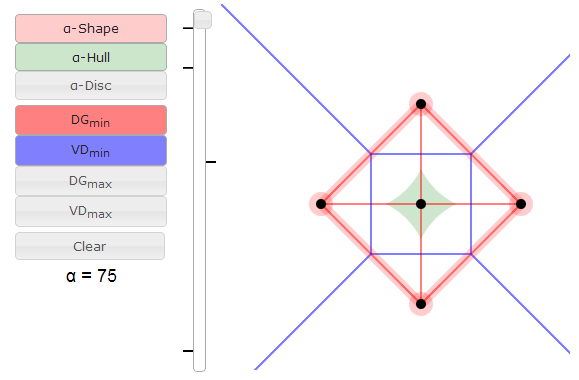
\includegraphics[scale=0.5]{../bilder/alphaShape_ui.png}
	\caption{Benutzeroberfläche der $\alpha$-Shapes HTML5-Applikation}
	\label{fig:alphaShape_ui}
\end{figure}

In Abbildung~\ref{fig:alphaShape_ui} ist die Benutzeroberfläche mit einigen aktivierten Anzeigemodi dargestellt.

Die Zeichenfläche besitzt zwei Eingabemodi. Der Punktmengenmodus ist aktiv, sofern der Anzeigemodus $\alpha$-Disc inaktiv ist. Im Punktmengenmodus können Punkte durch Links-Klick bzw. kurze Berührung eines Touchdisplays erstellt werden. Befindet sich im näheren Umkreises des Ereignisses schon ein Punkt, so wird dieser gelöscht. Durch Mouse- bzw. Touch-Drag-Ereignisse können Punkte verschoben werden. Mit dem Clear-Button können alle Punkte der Punktmenge gelöscht werden.

Im $\alpha$-Disc-Anzeige- und -Eingabemodus wird durch einen Links-Klick bzw. eine kurze Berührung der Mittelpunkt der $\alpha$-Disc verändert. Der Mittelpunkt kann auch durch Drag-Ereignisse verändert werden.

Der Parameter $\alpha$ kann über ein Slider-Steuerelement verändert werden. Auf einer Seite des Sliders befindet eine Markierung, welche dem Wert 0 entspricht. Auf der anderen Seite sind Markierungen angebracht, welche den Shape-Schwellen der Punktmenge entsprechen. Die Werte für $\alpha$ können mit einem Pixel Genauigkeit eingestellt werden.

\section{Mögliche Anwendungen}

Alle Anwendungen aus dem Kapitel über Shape-Spektrum-Algorithmen lassen sich mit der Applikation nachvollziehen. Für alle Beispiel-Probleme ist zu Beachten, dass sie nur im Rahmen der gegebenen Genauigkeit von einem Pixel gelöst werden können.

\begin{itemize}
\item Finden des dichtesten Paares: Ist der $\alpha$-Regler auf die kleinste, positive Markierung eingestellt, so sind die dichtesten Paare durch Kanten in der $\alpha$-Shape verbunden. Ein Beispiel dafür ist in Abbildung~\ref{fig:shapeHull_closestPair} dargestellt.

\item Finden des kleinsten einschließenden Kreises: Ist der $\alpha$-Regler auf die betragsmäßig kleinste, negative Markierung eingestellt, so ist der kleinste einschließende Kreis gleich dem Rand der $\alpha$-Hülle. Abbildung~\ref{fig:shapeHull_smallestCircle} stellt hierfür ein Beispiel dar.

\item Finden der konvexen Hülle: Ist der $\alpha$-Regler auf den größtmöglichen positiven oder negativen Wert eingestellt, so ist die $\alpha$-Hülle gleich der konvexen Hülle und die $\alpha$-Shape ist gleich dem Rand der konvexen Hülle. Auch hierzu gibt es ein Beispiel in Abbildung~\ref{fig:shapeHull_convex}.
\end{itemize}

Eine weitere mögliche Anwendung ist das Erkennen von Strukturen in verrauschten Bildern. Hierzu kann kein $\alpha$ angegeben werden, da diese Anwendung sehr von der Wahrnehmung des Benutzers abhängig ist.

\begin{figure}[htbp]
	\centering
	\subfloat[Verrauschtes Bild\label{fig:bigASNoise}]
		{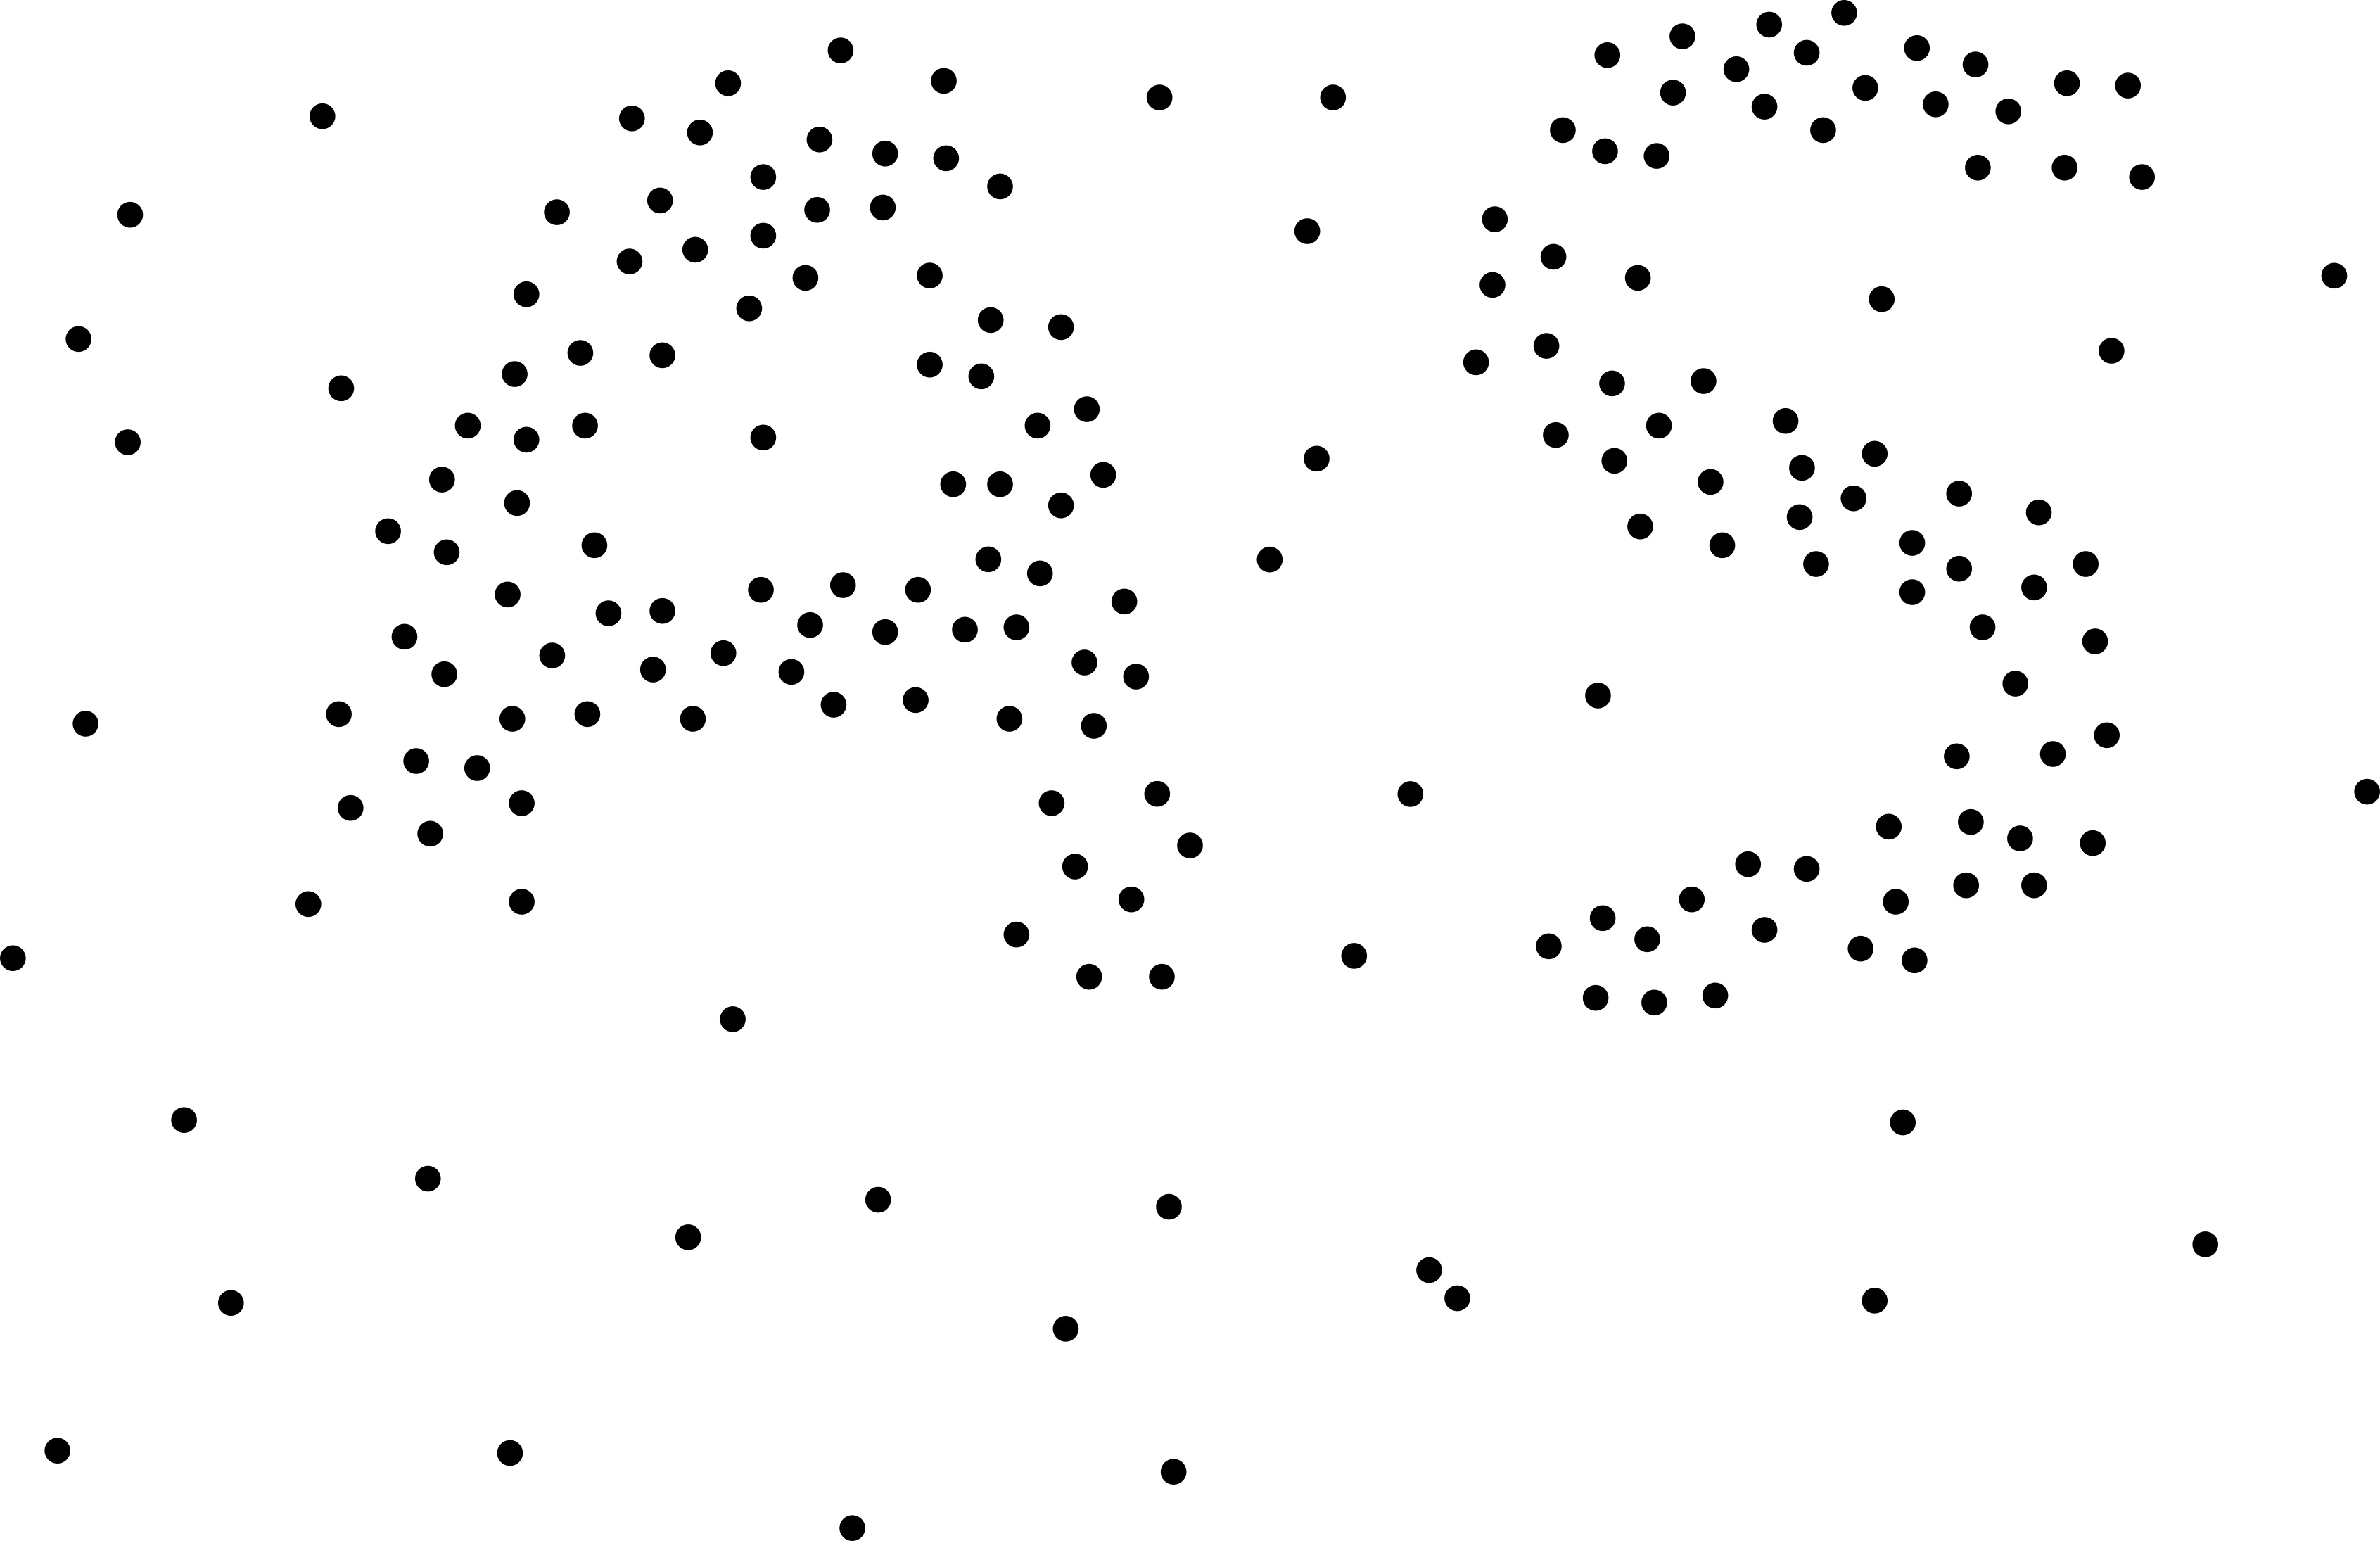
\includegraphics[scale=0.2]{../bilder/bigASNoise.png}}
	\hspace{2cm}
	\subfloat[Verrauschtes Bild mit $\alpha$-Shape\label{fig:bigASNoise_shape}]
		{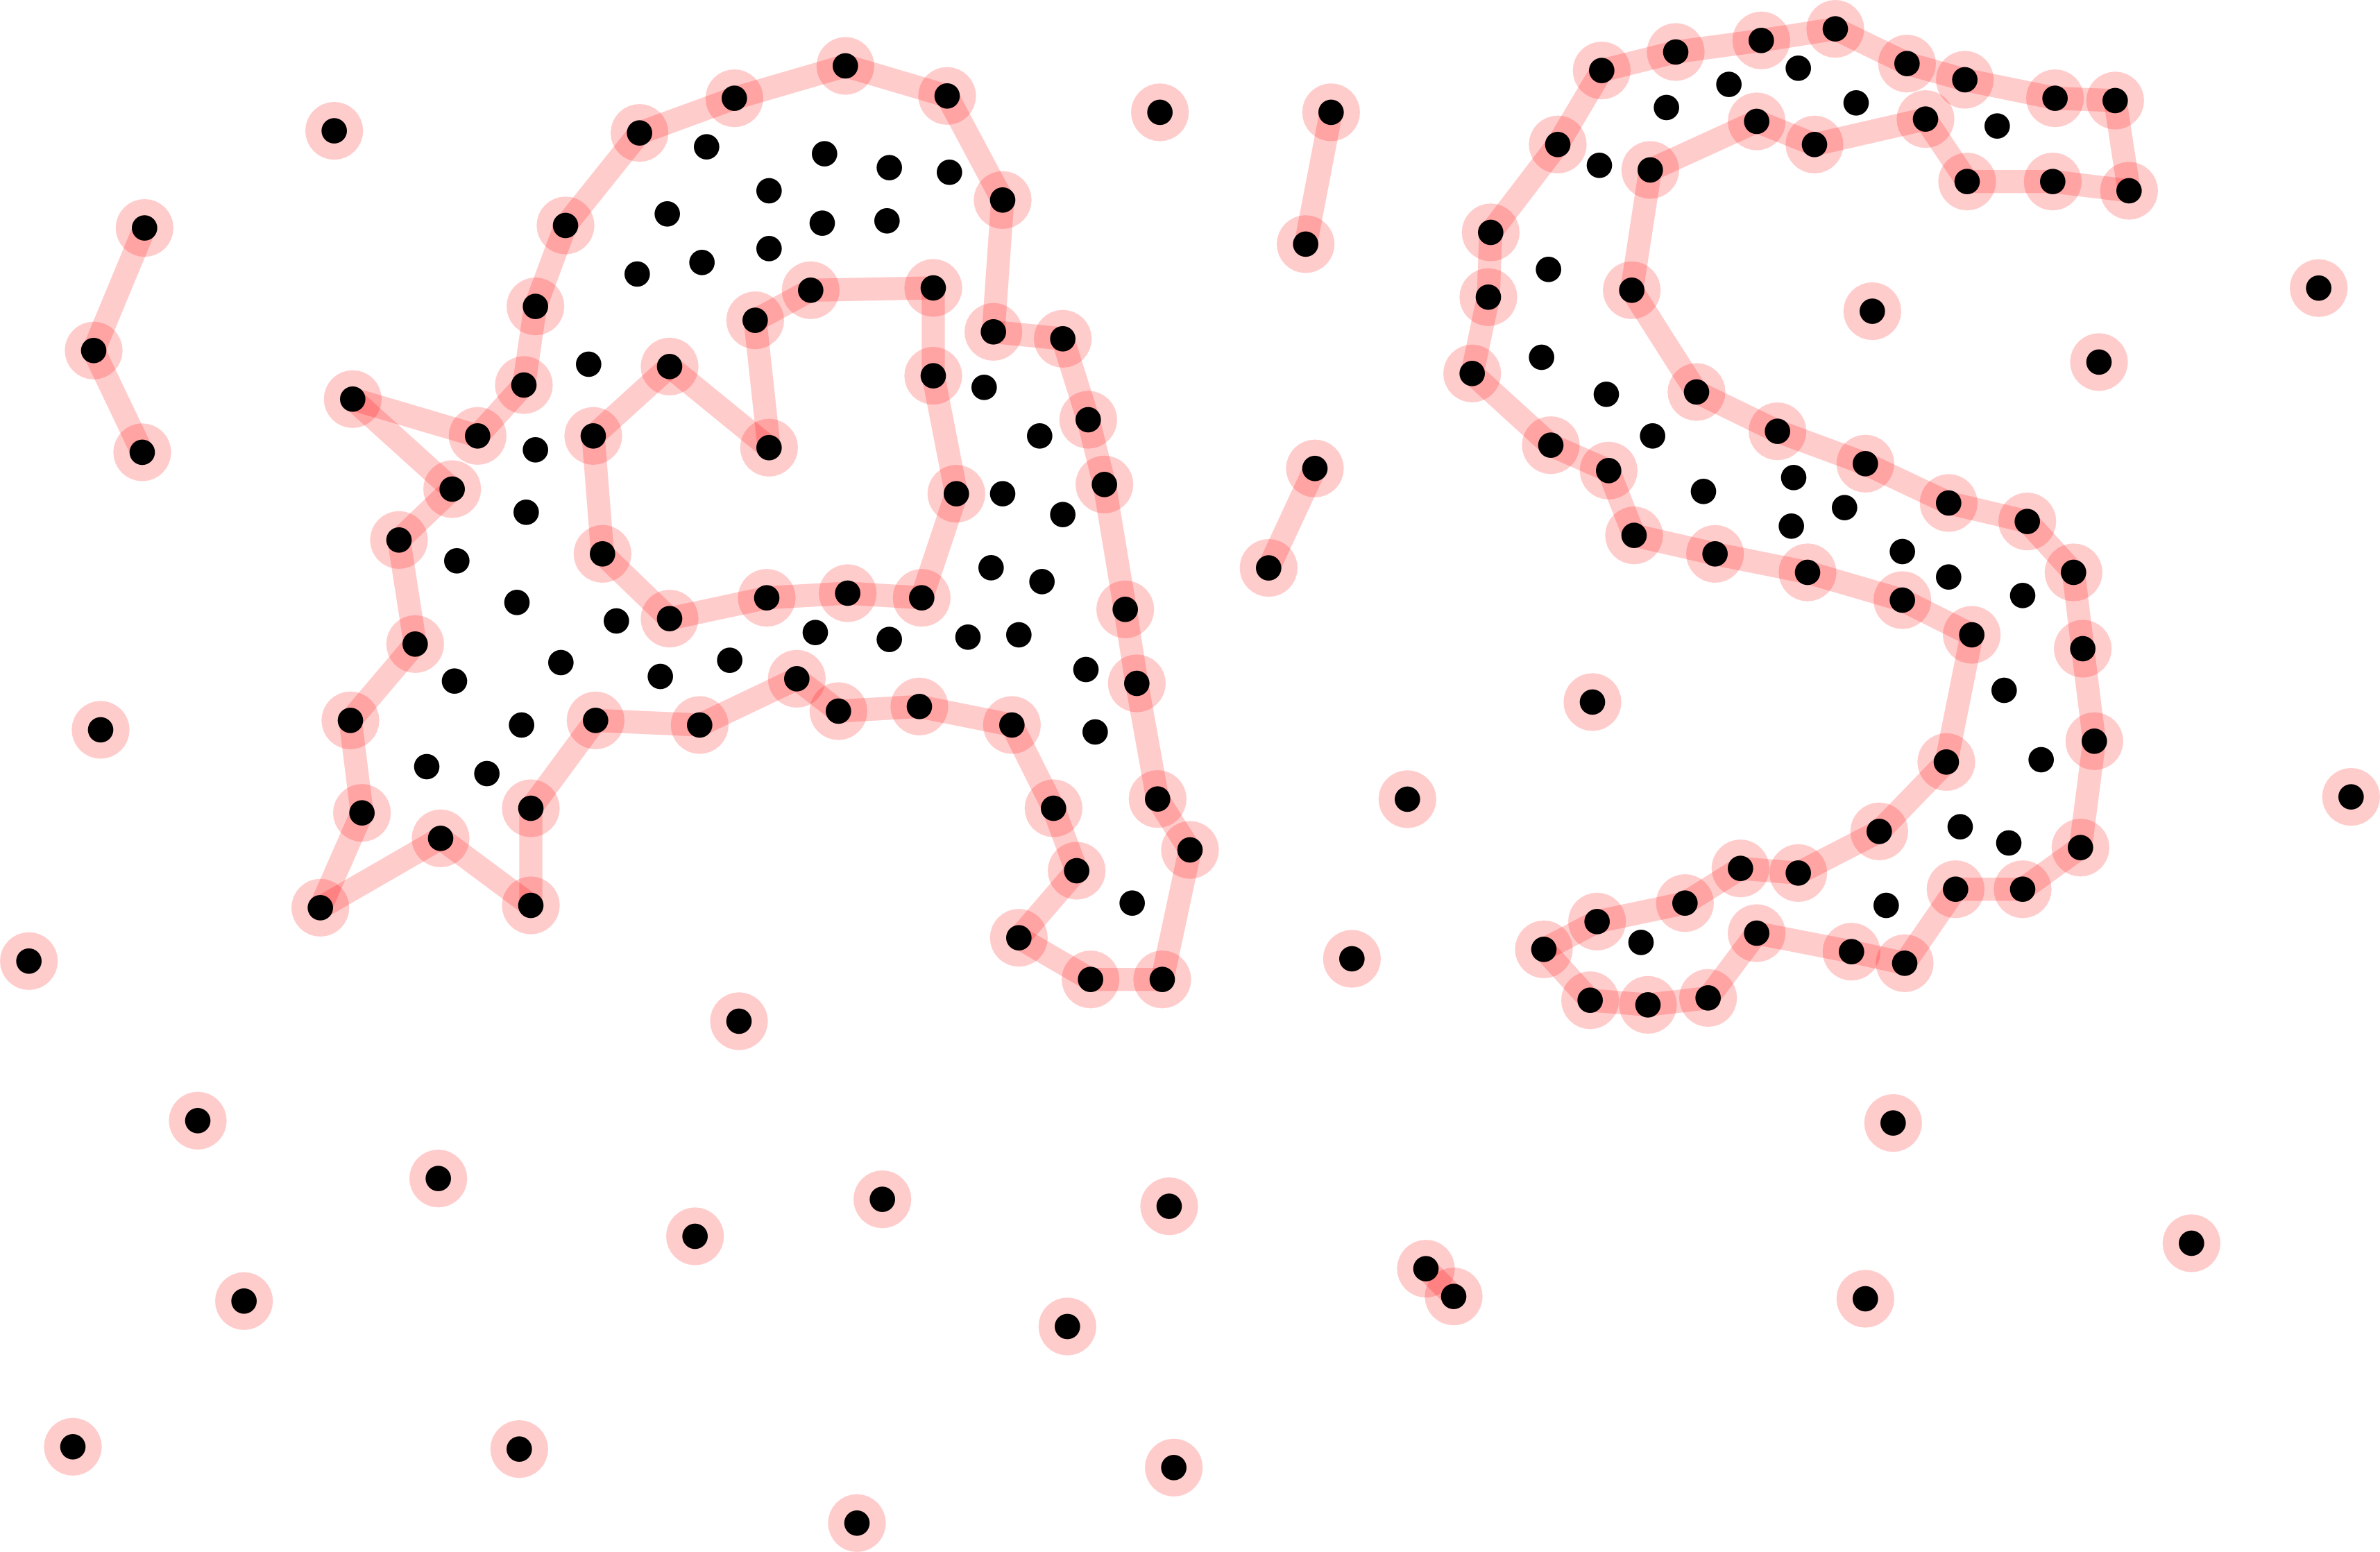
\includegraphics[scale=0.2]{../bilder/bigASNoise_shape.png}}
	\caption{Erkennung von Strukturen in verrauschten Bildern}
	\label{fig:pictureNoise}	
\end{figure}

Abbildung~\ref{fig:bigASNoise} zeigt das Beispiel der Gestalt der Buchstaben A und S. Hier wurden weitere Punkte eingefügt, welche als Rauschen interpretiert werden können. Abbildung~\ref{fig:bigASNoise_shape} zeigt die $\alpha$-Shape des verrauschten Bildes. Durch geschickte Wahl des Parameters $\alpha$ können $\alpha$-extreme Punkte mit Knotengrad 0 als Rauschen identifiziert werden. Die Erkennbarkeit der Buchstaben wird so deutlich erhöht.

Auch viele der in Kapitel \ref{alpha_props} gemachten Aussagen zu Eigenschaften von $\alpha$-Shapes können mit der Anwendung visualisiert werden. Hier seien nur ein paar Beispiele genannt.

\begin{itemize}
\item Die $\alpha$-Shape ist ein Subgraph des Delaunay-Graphen: Wählt man die Anzeigemodi $\alpha$-Shape, $DG_{\min}$ und $DG_{\max}$ aus und variiert $\alpha$ über den gesamten Wertebereich des Sliders, so kann man kann erkennen, dass jede Kante der Delaunay-Graphen für bestimmte $\alpha$ von einer Kante der $\alpha$-Shape überdeckt wird. Man kann auch erkennen, dass jede Kante der $\alpha$-Shape eine Kante eines Delaunay-Graphen überdeckt.

\item Man kann den eben beschriebenen Versuch auch getrennt für $DG_{\min}$ und positive $\alpha$ sowie für $DG_{\max}$ und negative $\alpha$ durchführen.

\item Bestimmung von $\alpha_{\max}$ für einen Knoten $P$ aus $DG_{\min}(S)$, welcher nicht auf dem Rand der konvexen Hülle liegt: Zu Beginn stellt man den Anzeigemodus $\alpha$-Shape ein und wählt $\alpha = 0$. Dann erhöht man $\alpha$ solange, bis $P$ nicht mehr rot umrandet ist. Der letzte angezeigte Wert von $\alpha$, für welchen $P$ noch rot umrandet war, ist $\lfloor \alpha_{\max} \rfloor$.

\item Bestimmen eines Knotens des Voronoi-Diagramms auf der Begrenzung von $VC_{\min}(P)$, welcher Abstand $\alpha_{\max}$ zu $P$ hat. $P$ darf dazu nicht auf dem Rand der konvexen Hülle liegen.  Hierzu werden zusätzlich zum letzten Versuch die Anzeigemodi $VD_{\min}$ und $\alpha$-Disc benötigt. Es muss $\alpha = \lfloor \alpha_{\max} \rfloor$ eingestellt werden. Dann wird der Mittelpunkt der $\alpha$-Disc nacheinander auf alle Knoten von $VD_{\min}(S)$, welche auf dem Rand von $VC_{\min}(P)$ liegen, platziert. Liegt $P$ für einen dieser Knoten auf dem Rand der Kreisscheibe, so ist ein Knoten mit Abstand $\alpha_{\max}$ zu $P$ gefunden.
\end{itemize} 

\section{Plattformspezifische Besonderheiten}

Da die Anwendung sowohl in einem Browser auf einem PC als auch auf mobilen Geräten, wie Smartphones oder Tablets, bedienbar sein soll, sind einige Dinge zu beachten.

Die Bedienelemente müssen groß genug sein um sie mit dem Finger bedienen zu können. Hierzu gibt es JavaScript-Bibliotheken, welche anpassbare Steuerelemente anbieten. Für die hier beschriebene Anwendung wurde die Bibliothek "`jQuery user interface"' benutzt, welche unter \autocite{jqueryui} zu finden ist. Alle Button-Steuerelement sowie der Slider stammen aus ihr. Für die Steuerelemente aus "`jQuery user interface"' sind die Event-Handler, welche eine Touchbedienung ermöglichen, nicht implementiert. Hierzu ist die Bibliothek "`jQuery UI Touch Punch"' notwendig, welche unter \autocite{jqueryuitouch} zu finden ist. Bei der Zeichenfläche ist darauf zu achten, selbst die Event-Handler für Mouse- und Touch-Events zu implementieren.

Weiterhin ist zu Beachten, dass mobile Geräte in der Anzeigegröße sehr eingeschränkt sind. Auch kann ein solches Gerät in zwei verschiedenen Ausrichtungen, Hoch- und Querformat, bedient werden. Auch ein Browser-Fenster auf einem PC kann verschiedene Größen sowie Hoch- und Querformat annehmen.

Wird diese Anwendung in einem Fenster im Querformat ausgeführt, so werden die Button- und Slider-Bedienelemente links und die Zeichenfläche rechts dargestellt. Die Buttons werden untereinander und der Slider wird rechts daneben, vertikal dargestellt. Hat das Fenster eine ausreichende Höhe, so werden alle Bedienelemente dargestellt. Ist die Höhe des Fensters kleiner als eine gewisse minimale Höhe, so werden die Bedienelemente für Delaunay-Graphen und Voronoi-Diagramme nicht dargestellt.

\begin{figure}[htbp]
	\centering
	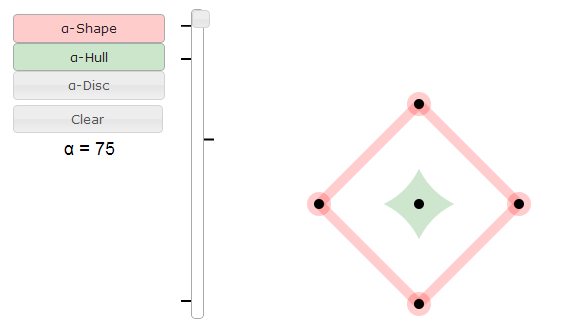
\includegraphics[scale=0.5]{../bilder/alphaShape_uiMin.png}
	\caption{Minimale Benutzeroberfläche der $\alpha$-Shapes HTML5-Applikation}
	\label{fig:alphaShape_uiMin}
\end{figure}

Abbildung~\ref{fig:alphaShape_uiMin} zeigt die Anwendung im Querformat mit ausgeblendeten Eingabemöglichkeiten.

Wird die Anwendung in einem Fenster im Hochformat ausgeführt, so werden nur die Buttons für $\alpha$-Shape, -Hülle, und -Kreisscheibe sowie der Slider dargestellt. Diese Bedienelemente werden oben dargestellt und die Zeichenfläche unten. Je nach Breite des Fensters werden die Buttons nebeneinander oder untereinander dargestellt. Der Slider wird unter den Buttons horizontal dargestellt.

\begin{figure}[htbp]
	\centering
	\subfloat[Darstellung im Hochformat\label{fig:alphaShape_uiVertNoBreak}]
		{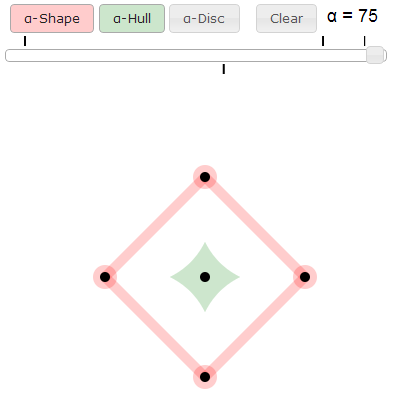
\includegraphics[scale=0.4]{../bilder/alphaShape_uiVertNoBreak.png}}
	\hspace{2cm}
	\subfloat[Darstellung im Hochformat mit Umbruch\label{fig:alphaShape_uiVertBreak}]
		{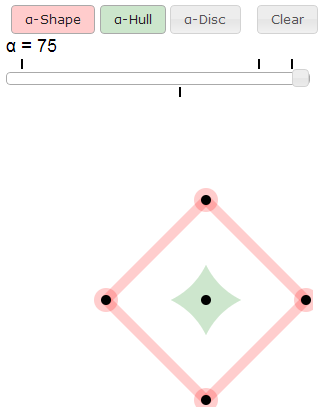
\includegraphics[scale=0.4]{../bilder/alphaShape_uiVertBreak.png}}
	\caption{Darstellung der Benutzeroberfläche im Hochformat}
	\label{fig:alphaShape_uiVert}	
\end{figure}

In Abbildung~\ref{fig:alphaShape_uiVert} wird die Benutzeroberfläche im Hochformat mit und ohne Umbruch der Anzeigeelemente dargestellt.

Wie diese plattformspezifischen Besonderheiten im einzelnen mit HTML5 realisiert werden ist im Anhang beschrieben. Dort wird auch auf Besonderheiten bei der Entwicklung mit JavaScript im Vergleich zu Java eingegangen.
